\begin{figure*}[!t]
\centering
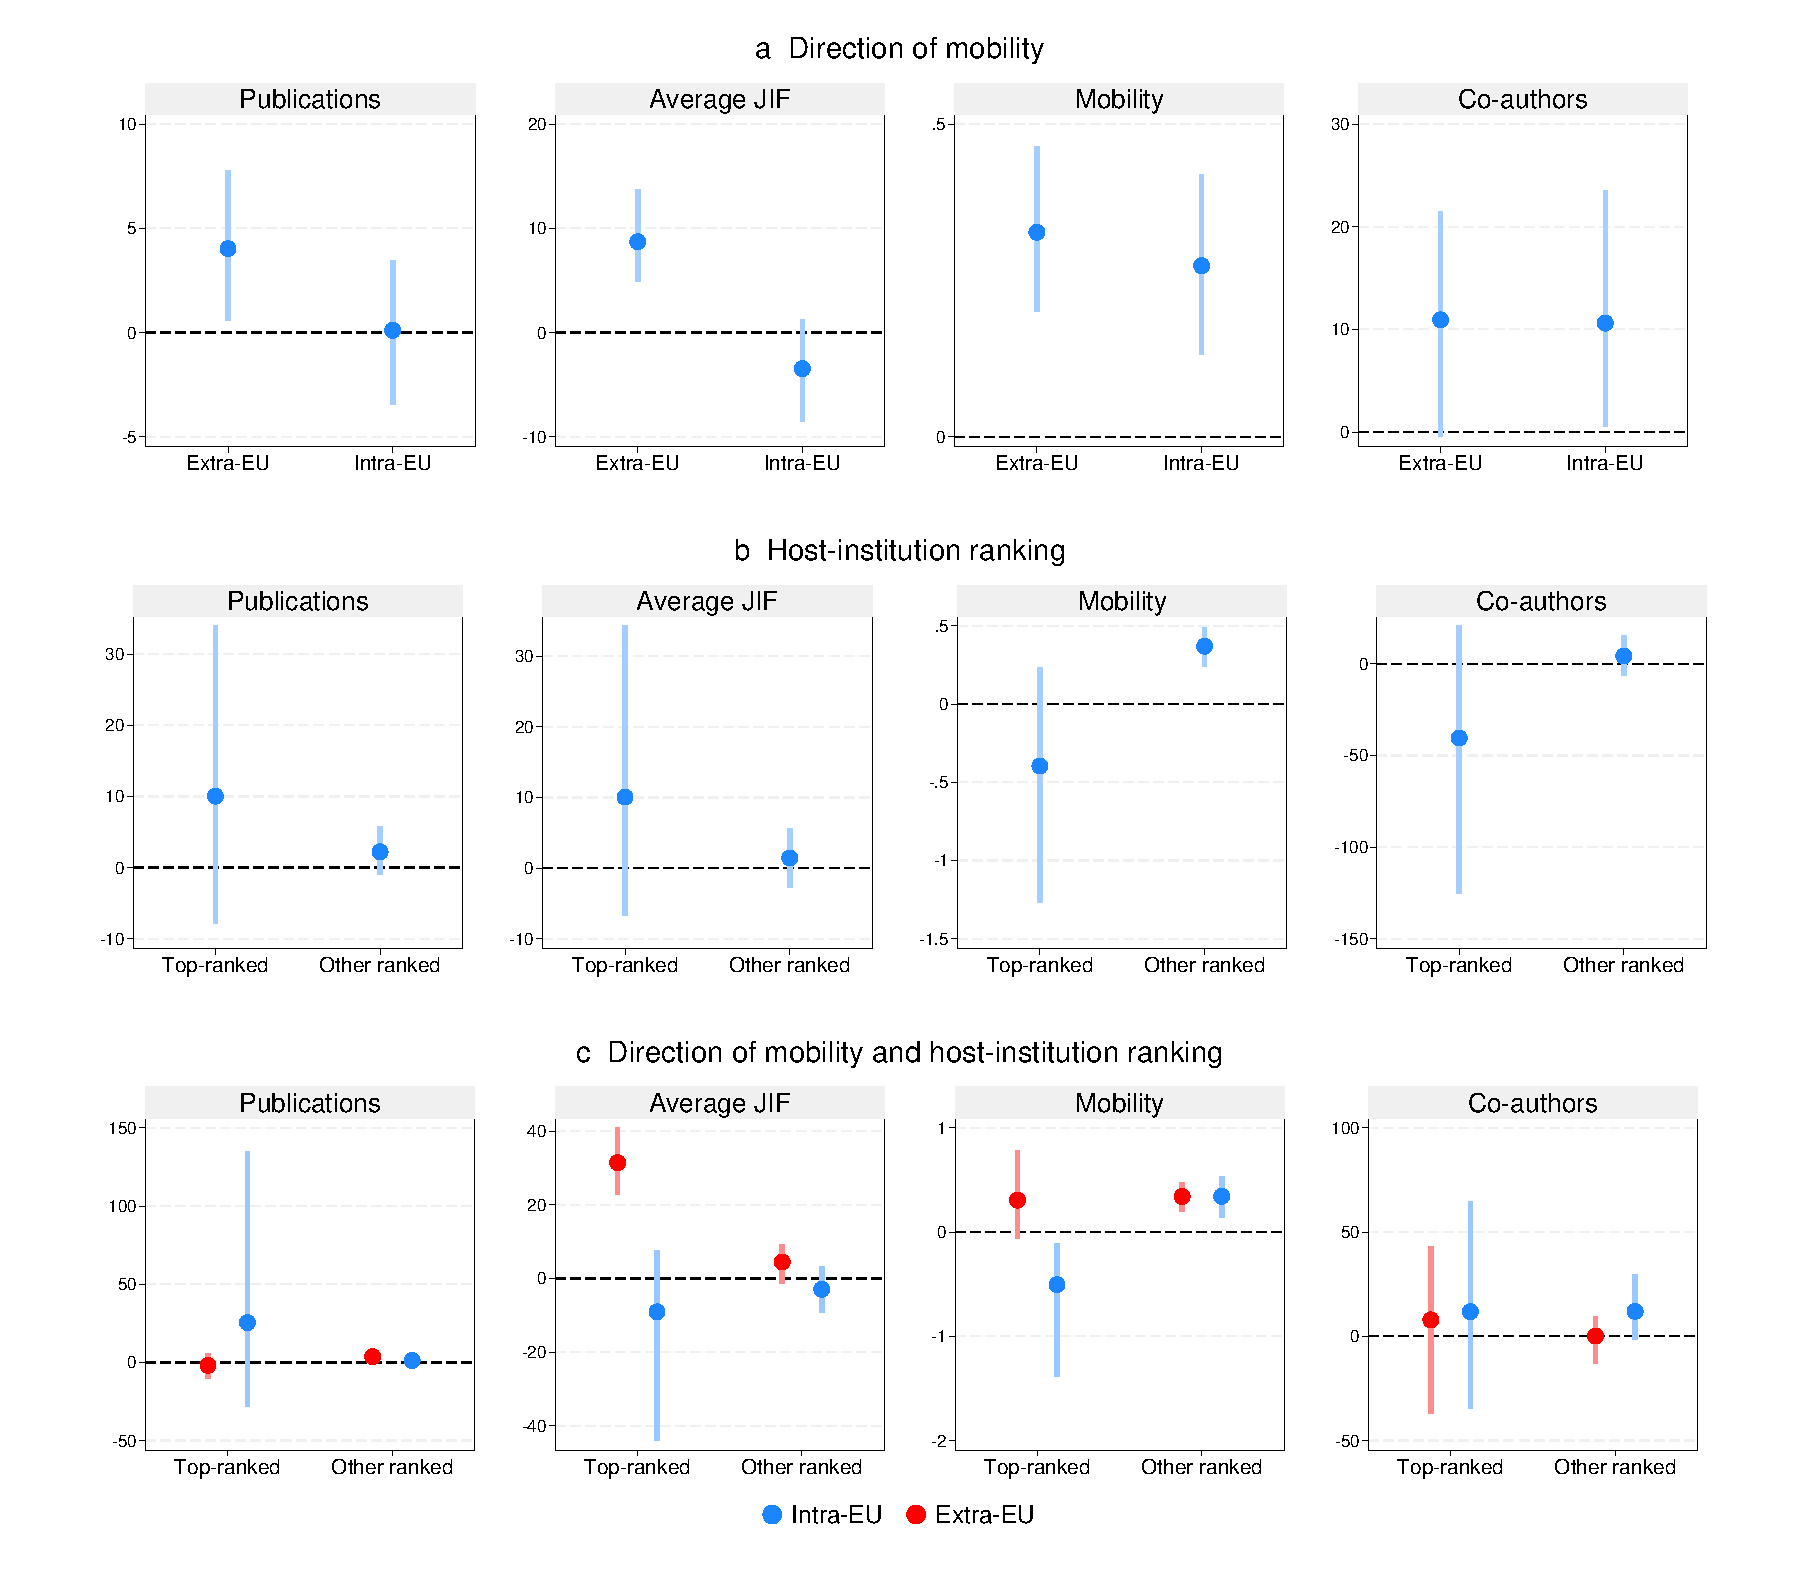
\includegraphics[width=1\textwidth]{output/figures/heterogeneity_combined.pdf}
\caption{\textbf{Effects by direction of mobility, host ranking, and their combination.} Five-year fuzzy regression-discontinuity estimates for publications, average JIF, intended-country affiliation (labelled ``Mobility''), and coauthor counts. Points are conventional estimates; lines are 90\% robust bias-corrected confidence intervals. (a) Within-EU mobility (labelled ``Intra-EU'') is mobility from one EU28 country to another EU28 country; extra-EU mobility is mobility from an EU28 country to a non-EU28 country or vice versa. EU28 membership includes the United Kingdom. (b) Institutions in the top 50 of the 2013 Scimago Institutions Rankings versus other ranked institutions. The labels ``Top-ranked'' and ``Other ranked'' refer to these ranking categories. (c) The four groups formed by crossing direction of mobility and host ranking; blue denotes Intra-EU and red denotes Extra-EU, as defined in panel a. Missing ranks are excluded in b and c. Specifications include separate local linear slopes, the pre-competition outcome, competition fixed effects, triangular kernels, outcome-specific mean-squared-error-optimal bandwidths, and competition-clustered inference.}
\label{fig:heterogeneity}
\end{figure*}
